\documentclass[12pt]{article}

\usepackage{sbc-template}

\usepackage{graphicx,url}

\usepackage[brazil]{babel} 
  
\usepackage[latin1]{inputenc}       

\sloppy

\title{Introdu\c c\~{a}o \`{a} Criptografia e algoritmo RSA}

\author{Henrique Shodi Maeta}


\address{{Centro Universit\'{a}rio Senac, Santo Amaro}
\email{japa1996@hotmail.com}}

\begin{document} 

\maketitle

\begin{abstract}
Transmit or receive confidential communication is not a recent necessity, and since antiquity it comes been developed new techniques of hidin and ciphering messages. Surrounded by many algorithms,  we will deal with, in this article, in particular the RSA, that is one of the most secure and used cryptography algorithm nowadays. 
  
\end{abstract}
     
\begin{resumo} 
Transmitir ou receber comunicados sigilosos n\~{a}o \'{e} uma necessidade recente, e desde a atinguidade  v\^{e}m sendo desenvolvidas novas t\'{e}cnicas de oculta\c c\~{a}o e cifragem de mensagens. Em meio \`{a} varios algoritmos trataremos neste artigo, em especial o RSA, que \'{e} um dos mais seguros e utilizados algoritmos de criptografia da atualidade.
\end{resumo}


\section{Introdu\c c\~{a}o}


 Transmitir ou receber mensagens sigilosas n\~{a}o \'{e} uma necessidade recente, h\'{a} relatos que na antiga Gr\'{e}cia eram utilizadas t\'{a}buas de madeiras, onde a mensagem era escrita, cobertas por cera, deste modo dificultaria o acesso e at\'{e} mesmo a consci\^{e}ncia de que a mensagem existia. Tamb\'{e}m, na Gr\'{e}cia antiga, dizem que um general raspava a cabe\c ca de um escravo e al\'{i} gravava uma mensagem. Quando o cabelo do escravo estivesse escondendo a mensagem ele era levado para o destinat\'{a}rio, e, essa t\'{e}cnica recebeu o nome de esteganografia. Por\'{e}m estas t\'{e}cnicas n\~{a}o eram muito eficientes, j\'{a} que se o escravo fosse interceptado por outra pessoa ou fosse retirada a cera da t\'{a}bua, n\~{a}o seria dif\'{i}cil achar estas mensagens. 
 
 Junto com a esteganografia uma outra t\'{e}cnica foi desenvolvida ao longo da hist\'{o}ria, tal t\'{e}cnica consistia em substituir cada letra da mensagem por uma outra letra, foi desenvolvida ent\~{a}o, a cifra Atbash dos Hebreus por volta de 600 a.c., onde a primeira letra do alfabeto deveria ser substitu\'{i}da pela ultima, a segunda pela penultima e assim por diante (Figura \ref{1} p\'{a}gina \pageref{1}).
\begin{figure}[!h]
\centering
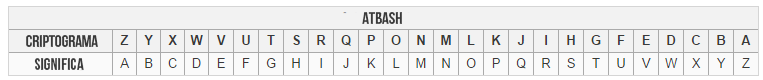
\includegraphics[scale = .5]{atbash}
\caption{Exemplo Cifra de Atbash}
\label{1}
\cite{gravity}
\end{figure}
 
  Alguns anos depois J\'{u}lio C\'{e}sar, l\'{i}der militar e pol\'{i}tico romano, inventou a cifra de C\'{e}sar, para se comunicar com seus generais de guerra, esta cifra consistia em deslocar o alfabeto uma determinada quantidade de vezes, e essa quantidade de vezes recebe o nome de chave, por exemplo, em uma mensagem encriptografada com a chave 1 na cifra de C\'{e}sar a letra A ser\'{a} substitu\'{i}da pela B, a B pela C e assim por diante (Figura \ref{2} p\'{a}gina \pageref{2}).
  

\begin{figure}[!h]
\centering
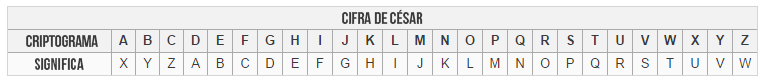
\includegraphics[scale = .5]{cesar}
\caption{Exemplo de Cifra de C\'{e}sar chave 3}
\label{2}
\cite{gravity}
\end{figure}
 \pagebreak
Estas t\'{e}cnicas de criptografia se manteram por muito tempo at\'{e} que Al-Kindi um matem\'{a}tico e fil\'{o}sofo \'{a}rabe iniciou uma discu\c c\~{a}o sobre t\'{e}cnicas de criptoan\'{a}lise. Al-Kindi expecificou que, conhecendo a linguagem em que foi escrita a mensagem, para decifr\'{a}-la poder\'{i}amos utilizar o metodo de letras prov\'{a}veis ou frequ\^{e}ntes (an\'{a}lise de frequ\^{e}ncia), por exemplo, um texto escrito em l\'{i}ngua portuguesa a frequ\^{e}ncia na qual a letra A aparece \'{e} muito alta, ent\~{a}o para decifrar o texto \'{e} necess\'{a}rio apenas verificar a const\^{a}ncia em que as letras aparecem e assim descobrir a chave que foi utilizada para encriptografar e, consequ\^{e}ntemente, descobrir o texto original.

 Por muitos anos foram sendo criadas novas maneiras de se encriptografar textos utilizando algoritmos de criptografia sim\'{e}trica, onde uma mesma chave pode tanto criptografar quanto descriptografar uma mensagem (Figura \ref{3} e Figura \ref{4}).
\begin{figure}[!h]
\centering
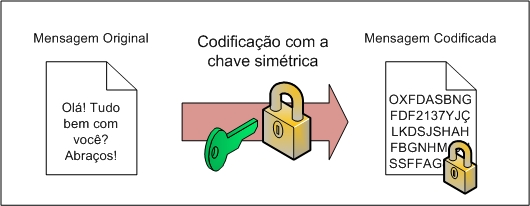
\includegraphics[scale = .5]{simetrica1}
\caption{Chave sim\'{e}trica usada para criptografar a mensagem}
\label{3}
\cite{ufrj}
\end{figure}

\begin{figure}[!h]
\centering
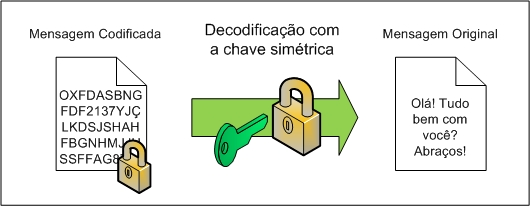
\includegraphics[scale = .5]{simetrica2}
\caption{Mesma chave usada, agora, para descriptografar a mensagem}
\label{4}
\cite{ufrj}
\end{figure}

Um exemplo de criptografia sim\'{e}trica \'{e} o algoritmo DES (Data Encryption Standard) com chave de 56 bits que foi criado pela IBM em 1977, por\'{e}m em um desafio promovido pela internet e utilizando-se do m\'{e}todo da tentativa e erro a seguran\c ca deste algoritmo foi quebrada. Por\'{e}m este tipo de criptografia tinha um problema: Como combinar uma chave privada entre duas pessoas que querem se comunicar pela internet? A solu\c c\~{a}o deste problema estava em um outro tipo de criptografia, a criptografia assim\'{e}trica que consiste em ter no m\'{i}nimo duas chaves, uma para criptografar e outra para descriptografar (Figura \ref{5} p\'{a}gina \pageref{5} e Figura \ref{6} p\'{a}gina \pageref{6}).
\begin{figure}[!h]
\centering
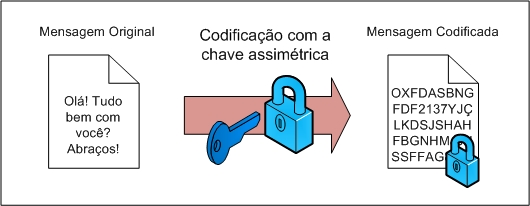
\includegraphics[scale = .5]{asimetrica1}
\caption{Chave azul para criptografar}
\label{5}
\cite{ufrj}
\end{figure}
\begin{figure}[!h]
\centering
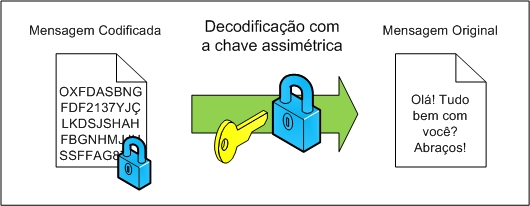
\includegraphics[scale = .5]{asimetrica2}
\caption{Chave amarela para descriptografar}
\label{6}
\cite{ufrj}
\end{figure}
\pagebreak

Ent\~{a}o, problema de chaves no algoritmo sim\'{e}trico foi resolvido, por\'{e}m um algoritmo assim\'{e}trico \'{e} muito mais demorado, fazendo com que o desenvolvedor tenha que fazer uma escolha s\'{a}bia, ponderando entre um algoritmo r\'{a}pido por\'{e}m n\~{a}o t\~{a}o seguro, ou, um algoritmo lento, por\'{e}m muito dif\'{i}cil de ser quebrado. 

Um algoritmo de criptografia assim\'{e}trica que se destacou foi o RSA, que \'{e} muito utilizado em transa\c c\~{o}es banc\'{a}rias, e-commerce, e v\'{a}rias \'{a}reas na qual a seguran\c ca da informa\c c\~{a}o \'{e} algo imprescind\'{i}vel, por conta da dificuldade de se obter a chave privada, mesmo sabendo como o algoritmo funciona.


 
\section{Algoritmo RSA}

Em 1978, tr\^{e}s professores do Massachusetts Institute of Technology(MIT) publicaram um artigo entitulado "A Method for Obtaining Digital Signatures and Public-Key Cryptosystems"\cite{rivest:1978} onde foi descrito um algoritmo para encriptografar e descriptografar uma mensagem utilizando n\'{u}meros primos na ordem de, aproximadamente, 600 d\'{i}gitos (como \'{e} recomendado, para que a seguran\c ca n\~{a}o falhe). Este algoritmo \'{e} muito seguro, pois \'{e} utilizado o produto de dois n\'{u}meros primos, e a dificuldade de se fatorar este produto e obter os primos utilizados \'{e} uma tarefa t\~{a}o ardua que para se descobrir os valores utilizados poderiam se levar anos, por conta de n\~{a}o possuirmos um algoritmo que nos fa\c ca este trabalho.

Para criptografar uma mensagem em RSA, devemos poder representar essa mensagem como um inteiro entre 0 e $n$ - 1 s\~{a}o necess\'{a}rios dois n\'{u}meros primos ($p$ e $q$, que dever\~{a}o ficar em segredo) o produto destes valores ir\'{a} gerar a chave p\'{u}blica $n$ ent\~{a}o:
\begin{center}
$n = p * q$
\end{center}

O pr\'{o}ximo passo \'{e} calcular $\varphi(n) = (p - 1) * (q - 1)$ para podermos determinar a chave privada $d$ que \'{e} determinada por:
\begin{center}
mdc($d$, $\varphi$) = 1
\end{center}
Ou seja, $d$ e $\varphi(n)$ dever\~{a}o ser primos entre si.

Sabendo $d$, o pr\'{o}ximo passo \'{e} calcular a chave p\'{u}blica $e$ que \'{e} dada por:
\begin{center}
$e * d$ mod $\varphi(n)$ = 1
\end{center}

Tendo os valores de $e, n$ e $d$, podemos ent\~{a}o criptografar mensagens utilizando as chaves p\'{u}blicas da seguinte maneira:
\begin{center}
$M^e$ mod $n$ = $C$
\end{center}
Onde $M$ \'{e} a mensagem original, e $C$ a mensagem cifrada. Para obtermos o texto original a partir do texto cifrado devemos utlizar:
\begin{center}
$C^d$ mod $n$ = $M$
\end{center}
\section{Conclus\~{a}o}
Desta forma podemos provar que o algoritmo RSA \'{e} muito seguro por conta da dificuldade de se obter os primos pela fatora\c c\~{a}o de seu produto e que tal dificuldade pode ser motivo para utilizar este algoritmo em aplicativos banc\'{a}rios, e-commerce, e-mails importantes entre outras muitas coisas, por\'{e}m por trabalhar com n\'{u}meros extensos a dificuldade de se computar estes dados aumenta de forma substancial, fazendo com que este algoritmo exija uma capacidade de processamento muito alta, pois caso contr\'{a}rio o processo pode se tornar muito demorado.


\bibliographystyle{sbc}
\bibliography{sbc-template}
\nocite{al-kadi:00}
\nocite{ufcg:02}
\nocite{oliveira2012criptografia}
\nocite{tech}
\nocite{ita}
\nocite{bruno}
\end{document}

%The origins of cryptology
%https://www.vivaolinux.com.br/artigo/Introducao-a-criptografia
%http://www.gta.ufrj.br/grad/09_1/versao-final/stegano/introducao.html
%http://www.dsc.ufcg.edu.br/~pet/jornal/abril2014/materias/historia_da_computacao.html
%http://www.ronielton.eti.br/publicacoes/artigorevistasegurancadigital2012.pdf